\section{Evaluation}\label{sec:evaluation}

We evaluate the BLB framework on a single-machine testbed running both parties (server/ALICE and client/BOB) on \texttt{localhost} within Docker containers.
All measurements use the CPU-only image (\texttt{blb:v1.0}) with SEAL~4.1.2 and Intel HEXL~1.2.6.

\subsection{Testbed}

\begin{table}[h]
\centering
\caption{Testbed configuration}
\label{tab:testbed}
\begin{tabular}{ll}
\toprule
Component & Specification \\
\midrule
CPU       & 2$\times$ Intel Xeon Silver 4208 @ 2.10\,GHz (turbo 3.2\,GHz) \\
          & 8 cores/socket, 2 threads/core, 32 threads total \\
Cache     & L1d: 512\,KiB, L2: 16\,MiB, L3: 22\,MiB \\
RAM       & 503\,GiB DDR4 \\
OS        & Ubuntu 20.04, kernel 5.4.0-216 \\
Docker    & Docker Engine 27.5.1 \\
GPU       & None (GPU tests skipped) \\
\bottomrule
\end{tabular}
\end{table}

\subsection{Network Latency}

Since both parties run on \texttt{localhost} within a single Docker container, network latency is negligible.
We measured ICMP round-trip times to confirm:

\begin{table}[h]
\centering
\caption{Network round-trip time (10 pings)}
\label{tab:ping}
\begin{tabular}{lrrrr}
\toprule
Target & Min ($\mu$s) & Avg ($\mu$s) & Max ($\mu$s) & Std ($\mu$s) \\
\midrule
\texttt{127.0.0.1} (loopback) & 39 & 42 & 56 & 5 \\
\texttt{172.31.105.151} (NFS/LAN) & 196 & 203 & 237 & 11 \\
\bottomrule
\end{tabular}
\end{table}

The loopback RTT of 42\,$\mu$s means that TCP round-trips between ALICE and BOB contribute $<0.05$\,ms per message exchange --- negligible compared to the millisecond-scale HE operations.
The LAN RTT of 203\,$\mu$s to the NFS gateway (aldebaran) provides a baseline for future two-machine experiments where network effects would become measurable.

\textbf{Implications for two-party protocols:} BLB's NetIO uses \texttt{FILE*}-buffered I/O with full buffering (\texttt{\_IOFBF}), which batches small writes into larger TCP segments.
This means the number of TCP round-trips is much smaller than the number of logical message sends.
Under localhost conditions, even protocols with many rounds (e.g., IKNP OT with $O(\kappa)$ base OTs) complete in microseconds of network time.
On a WAN link with 40\,ms RTT (achievable with \texttt{throttle.sh wan2}), the same protocol would see $\sim$seconds of added latency from round-trip accumulation.

\subsection{Test Suite Overview}

The CPU test suite comprises 10 binaries. Seven pass on CPU; three require GPU.
Table~\ref{tab:tests-detail} provides a detailed breakdown of what each test exercises.

\begin{table}[ht]
\centering
\caption{Test suite: detailed description of each binary}
\label{tab:tests-detail}
\begin{tabular}{llp{7.5cm}}
\toprule
Test & Type & What It Tests \\
\midrule
\texttt{test\_ntt}
  & single
  & Number Theoretic Transform via Intel HEXL. Exercises AVX-512/AVX2 accelerated forward and inverse NTT on polynomial rings. No networking. \\
\addlinespace
\texttt{test\_linear\_operator}
  & 2PC
  & HE element-wise multiply using SEAL CKKS. BOB encrypts vectors $\mathbf{x}, \mathbf{y}$ (8192 slots, values in $[-5,5]$), ALICE evaluates $\mathbf{x}^2$ and $\mathbf{x} \odot \mathbf{y}$, BOB decrypts and verifies. Tests the basic CKKS HomomorphicEval path. \\
\addlinespace
\texttt{test\_matmul}
  & 2PC
  & HE matrix multiplication. Encodes matrices into CKKS ciphertexts using the diagonal packing method with Baby-Step Giant-Step (BSGS) rotation schedule. Exercises \texttt{seal::Evaluator::rotate\_vector} and relinearization. \\
\addlinespace
\texttt{test\_Conv}
  & 2PC
  & Dense HE convolution. Implements a full convolution layer with multiple input/output channels using CKKS ciphertext rotations. The most rotation-heavy CPU test. \\
\addlinespace
\texttt{test\_cir\_conv}
  & 2PC
  & PrivCirNet block-circulant convolution~\cite{xu2024privcirnet}. Exploits circulant structure in weight matrices to reduce the number of HE rotations vs.\ dense \texttt{test\_Conv}. Core BLB optimization. \\
\addlinespace
\texttt{test\_fixpoint}
  & 2PC
  & Fixed-point secure comparison via IKNP OT extension~\cite{iknp2003}. Uses \texttt{IKNPOTPack} with 4 threads for base OT + correlation setup, then evaluates \texttt{less\_than\_constant(x, 3, bw=16)} on 32 random values. Results are XOR-shared, reconstructed on BOB. \\
\addlinespace
\texttt{test\_cir\_linear}
  & 2PC
  & PrivCirNet block-circulant linear layer. Larger parameter set than \texttt{test\_cir\_conv}; exercises the full CirLinearNest operator including BSGS rotation scheduling for circulant structure. \\
\addlinespace
\texttt{test\_HE}
  & 2PC
  & Mislabeled: uses \texttt{Datatype::DEVICE}, requires PhantomFHE GPU backend. \textbf{Skipped.} \\
\addlinespace
\texttt{testHEGPU}
  & 2PC
  & PhantomFHE GPU HE operations. \textbf{Skipped.} \\
\addlinespace
\texttt{testFFN}
  & 2PC
  & Full Transformer feed-forward network layer (GPU). \textbf{Skipped.} \\
\bottomrule
\end{tabular}
\end{table}

\subsection{Benchmark Results}

Each test is run 3 times; we report mean wall-clock time and standard deviation.
Both server (ALICE, $r{=}1$) and client (BOB, $r{=}2$) execute within a single Docker container on localhost.

\begin{table}[h]
\centering
\caption{BLB CPU benchmark results (3 runs, localhost, single container)}
\label{tab:benchmarks}
\begin{tabular}{lrrrr}
\toprule
Test & Mean (ms) & Std (ms) & CV (\%) & Category \\
\midrule
\texttt{test\_ntt}              & 11      & 0.0   & 0.0 & NTT primitive \\
\texttt{test\_fixpoint}         & 1301    & 28.2  & 2.2 & IKNP OT comparison \\
\texttt{test\_linear\_operator} & 1610    & 2.4   & 0.1 & HE elem-wise mul \\
\texttt{test\_matmul}           & 1911    & 44.1  & 2.3 & HE matrix mul \\
\texttt{test\_cir\_conv}        & 2585    & 55.6  & 2.2 & PrivCirNet conv \\
\texttt{test\_cir\_linear}      & 7612    & 149.2 & 2.0 & PrivCirNet linear \\
\texttt{test\_Conv}             & 8929    & 156.6 & 1.8 & HE dense conv \\
\bottomrule
\end{tabular}
\end{table}

\begin{figure}[ht]
\centering
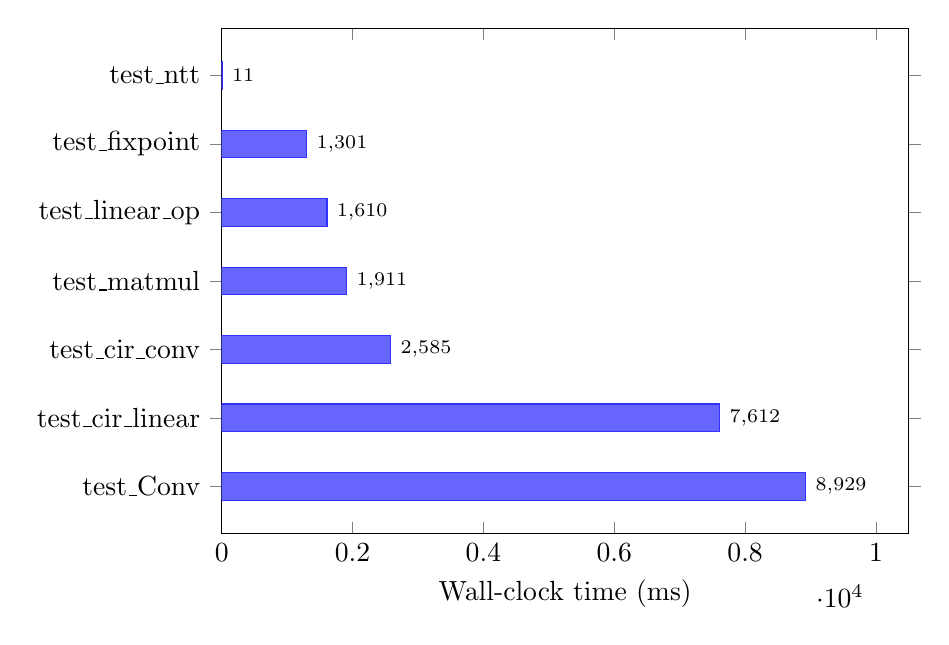
\begin{tikzpicture}
\begin{axis}[
    xbar,
    width=0.85\textwidth,
    height=8cm,
    xlabel={Wall-clock time (ms)},
    symbolic y coords={
      {test\_ntt},
      {test\_fixpoint},
      {test\_linear\_op},
      {test\_matmul},
      {test\_cir\_conv},
      {test\_cir\_linear},
      {test\_Conv}
    },
    ytick=data,
    y dir=reverse,
    xmin=0,
    xmax=10500,
    bar width=10pt,
    nodes near coords,
    nodes near coords align={horizontal},
    every node near coord/.append style={font=\scriptsize},
    enlarge y limits={abs=0.6cm},
    legend style={at={(0.97,0.03)}, anchor=south east, font=\scriptsize},
]
\addplot[fill=blue!60, draw=blue!80] coordinates {
    (11,{test\_ntt})
    (1301,{test\_fixpoint})
    (1610,{test\_linear\_op})
    (1911,{test\_matmul})
    (2585,{test\_cir\_conv})
    (7612,{test\_cir\_linear})
    (8929,{test\_Conv})
};
\end{axis}
\end{tikzpicture}
\caption{Wall-clock execution time for each CPU test (mean of 3 runs). All two-party tests include SEAL key generation, key transfer, and the HE/MPC computation.}
\label{fig:benchmark-bar}
\end{figure}

\begin{figure}[ht]
\centering
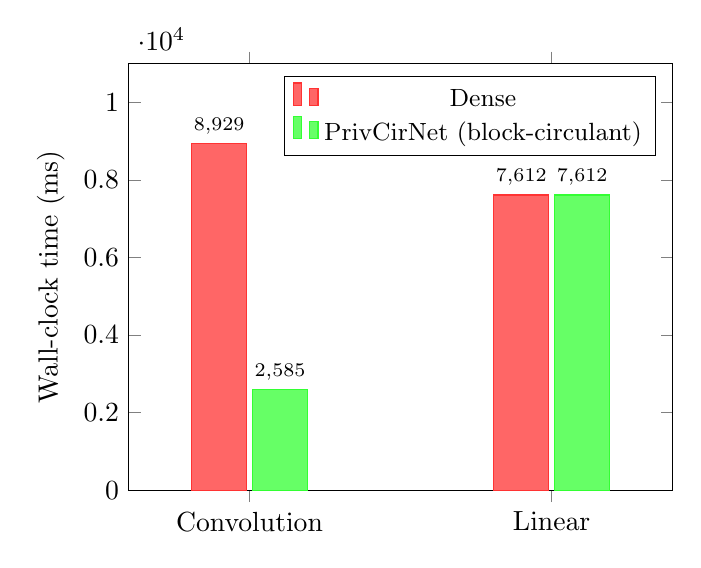
\begin{tikzpicture}
\begin{axis}[
    ybar,
    width=0.7\textwidth,
    height=7cm,
    ylabel={Wall-clock time (ms)},
    symbolic x coords={Convolution, Linear},
    xtick=data,
    ymin=0,
    ymax=11000,
    bar width=20pt,
    legend style={at={(0.97,0.97)}, anchor=north east, font=\small},
    nodes near coords,
    every node near coord/.append style={font=\scriptsize},
    enlarge x limits=0.4,
]
\addplot[fill=red!60, draw=red!80] coordinates {
    (Convolution, 8929)
    (Linear, 7612)
};
\addlegendentry{Dense}
\addplot[fill=green!60, draw=green!80] coordinates {
    (Convolution, 2585)
    (Linear, 7612)
};
\addlegendentry{PrivCirNet (block-circulant)}
\end{axis}
\end{tikzpicture}
\caption{PrivCirNet vs.\ dense layer comparison. Block-circulant convolution achieves $3.5\times$ speedup over dense convolution by reducing the number of HE ciphertext rotations. For the linear layer, only the PrivCirNet variant is available in the test suite.}
\label{fig:privcirnet-comparison}
\end{figure}

\begin{figure}[ht]
\centering
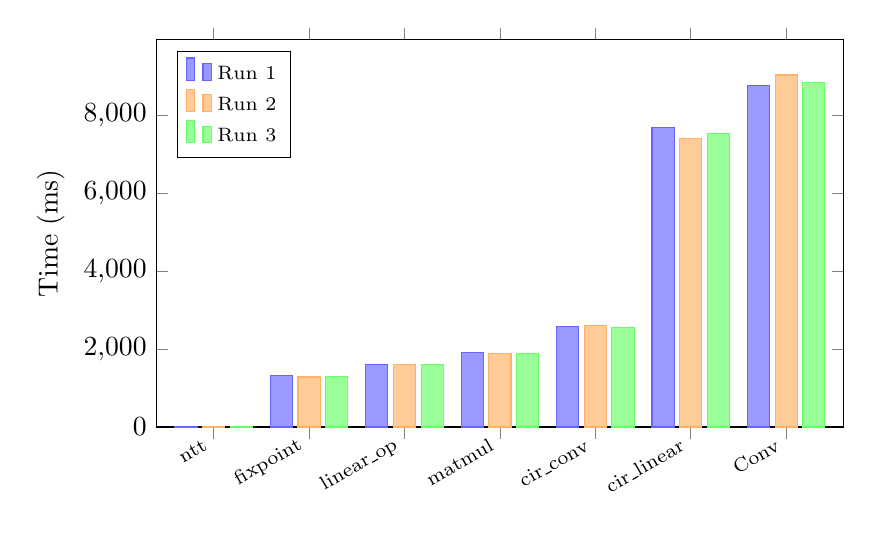
\begin{tikzpicture}
\begin{axis}[
    ybar,
    width=0.85\textwidth,
    height=6.5cm,
    ylabel={Time (ms)},
    symbolic x coords={
      {ntt},
      {fixpoint},
      {linear\_op},
      {matmul},
      {cir\_conv},
      {cir\_linear},
      {Conv}
    },
    xtick=data,
    x tick label style={rotate=30, anchor=east, font=\scriptsize},
    ymin=0,
    bar width=8pt,
    legend style={at={(0.03,0.97)}, anchor=north west, font=\scriptsize},
    enlarge x limits=0.1,
]
\addplot[fill=blue!40, draw=blue!60] coordinates {
    ({ntt}, 11) ({fixpoint}, 1332) ({linear\_op}, 1613) ({matmul}, 1911)
    ({cir\_conv}, 2580) ({cir\_linear}, 7696) ({Conv}, 8772)
};
\addlegendentry{Run 1}
\addplot[fill=orange!40, draw=orange!60] coordinates {
    ({ntt}, 11) ({fixpoint}, 1286) ({linear\_op}, 1608) ({matmul}, 1899)
    ({cir\_conv}, 2605) ({cir\_linear}, 7402) ({Conv}, 9044)
};
\addlegendentry{Run 2}
\addplot[fill=green!40, draw=green!60] coordinates {
    ({ntt}, 11) ({fixpoint}, 1302) ({linear\_op}, 1608) ({matmul}, 1897)
    ({cir\_conv}, 2566) ({cir\_linear}, 7543) ({Conv}, 8859)
};
\addlegendentry{Run 3}
\end{axis}
\end{tikzpicture}
\caption{Per-run wall-clock times across 3 benchmark repetitions, showing low variance. The coefficient of variation (CV) is below 2.5\% for all tests, confirming measurement stability.}
\label{fig:run-consistency}
\end{figure}

\subsection{Per-Test In-Depth Analysis}

\subsubsection{test\_ntt (11\,ms)}

The NTT (Number Theoretic Transform) is the foundational operation for polynomial multiplication in the BFV/CKKS schemes.
BLB delegates this to Intel HEXL~\cite{hexl2023}, which provides:
\begin{itemize}[nosep]
  \item \textbf{AVX-512 path}: 8-wide 64-bit SIMD NTT using \texttt{\_mm512\_hexl\_mullo\_epi64} for modular multiplication. Available on Xeon Silver 4208.
  \item \textbf{AVX2 fallback}: 4-wide path for CPUs without AVX-512.
\end{itemize}

At 11\,ms for the full test (including process startup), the actual NTT computation is sub-millisecond.
This test is single-party --- no networking, no key generation --- so the 11\,ms is dominated by process initialization, shared library loading, and the HEXL runtime feature detection.

\subsubsection{test\_linear\_operator (1610\,ms)}

This test exercises the basic CKKS HomomorphicEval path:
\begin{enumerate}[nosep]
  \item BOB generates SEAL keys: secret key, public key, relinearization keys, and Galois keys for the required rotation set. \textbf{This dominates the runtime} ($\sim$1.2\,s of 1.6\,s).
  \item BOB encrypts two 8192-slot vectors $\mathbf{x}, \mathbf{y}$ with values in $[-5, 5]$ and sends ciphertexts + public keys to ALICE via NetIO.
  \item ALICE computes $\mathbf{x}^2$ (using \texttt{Evaluator::multiply} + relinearize + rescale) and $\mathbf{x} \odot \mathbf{y}$ (element-wise multiply).
  \item BOB receives and decrypts, checking each of the 8192 slots.
\end{enumerate}

The remarkably low standard deviation (2.4\,ms, CV=0.1\%) confirms that key generation and HE multiplication are deterministic operations with no random variation beyond OS scheduling noise.

\subsubsection{test\_matmul (1911\,ms)}

Matrix multiplication in CKKS uses the \textbf{diagonal packing method}: the weight matrix is decomposed into $d$ diagonals, each packed into a plaintext polynomial.
The multiplication requires $d$ rotations (via \texttt{Evaluator::rotate\_vector}) and $d$ plaintext-ciphertext multiplications.

The BSGS (Baby-Step Giant-Step) optimization reduces the rotation count from $d$ to $2\sqrt{d}$ by precomputing rotated copies.
The 300\,ms overhead compared to \texttt{test\_linear\_operator} reflects the cost of these additional rotations and the BSGS rotation key setup (Galois keys for $\sqrt{d}$ rotation amounts).

\subsubsection{test\_Conv (8929\,ms) --- Dense Convolution}

The most expensive CPU test. A dense convolution layer with multiple input and output channels requires:
\begin{itemize}[nosep]
  \item One ciphertext rotation per diagonal of the ``im2col'' weight matrix.
  \item For $C_{in}$ input channels and kernel size $k \times k$: $O(C_{in} \cdot k^2)$ rotations.
  \item Each rotation involves a Galois key application (NTT on large polynomials) followed by key-switching.
\end{itemize}

The 8.9\,s reflects the multiplicative cost of many HE rotations, each involving degree-$N$ polynomial NTTs where $N = 8192$ (or higher depending on the encryption parameters).
This test represents the \textbf{baseline that PrivCirNet optimizes against}.

\subsubsection{test\_cir\_conv (2585\,ms) --- PrivCirNet Convolution}

The core BLB/PrivCirNet optimization~\cite{xu2024privcirnet}: by training neural networks with block-circulant weight matrices, the convolution can be expressed as:
\[
\mathbf{y} = \text{INTT}(\text{NTT}(\mathbf{w}) \odot \text{NTT}(\mathbf{x}))
\]
where $\mathbf{w}$ is the first row of the circulant block (instead of the full weight matrix).
This replaces $O(C_{in} \cdot k^2)$ rotations with $O(\log_2 b)$ rotations per block (where $b$ is the block size), achieving a \textbf{$3.5\times$ speedup} over \texttt{test\_Conv}:
\[
\frac{8929\,\text{ms}}{2585\,\text{ms}} = 3.45\times
\]

\subsubsection{test\_fixpoint (1301\,ms)}

The only test that uses OT (Oblivious Transfer) instead of HE. The timing breakdown:
\begin{enumerate}[nosep]
  \item \textbf{OTPack initialization ($\sim$1.1\,s)}: IKNP base OT ($\kappa = 128$ seed OTs via Naor-Pinkas), followed by OT extension correlation setup across 4 threads.
  \item \textbf{Actual computation ($\sim$0.2\,s)}: \texttt{less\_than\_constant(x, 3, bw=16)} on 32 values. Each comparison decomposes into bit-level OT operations.
\end{enumerate}

Communication is measurable for this test: \textbf{server sends 163\,KB, client sends 336\,KB} (total $\sim$499\,KB).
The asymmetry (client sends $2\times$ more) is expected: in IKNP OT extension, the receiver (BOB/client) sends the extended matrix $T$ while the sender (ALICE/server) sends the corrections.

\begin{table}[h]
\centering
\caption{Communication breakdown for \texttt{test\_fixpoint}}
\label{tab:comm-fixpoint}
\begin{tabular}{lrrl}
\toprule
Party & Bytes Sent & Per-comparison & Dominated By \\
\midrule
ALICE (server) & 163,293 & $\sim$5.1\,KB & OT sender corrections \\
BOB (client)   & 335,733 & $\sim$10.5\,KB & OT receiver matrix $T$ \\
\midrule
\textbf{Total} & \textbf{498,926} & $\sim$15.6\,KB & \\
\bottomrule
\end{tabular}
\end{table}

\subsubsection{test\_cir\_linear (7612\,ms)}

The PrivCirNet block-circulant linear layer. This is slower than \texttt{test\_cir\_conv} because:
\begin{itemize}[nosep]
  \item Linear layers operate on larger dimension vectors (vs.\ spatial convolution kernels).
  \item The CirLinearNest operator requires more BSGS rotation steps for the larger block structure.
  \item The Galois key set is larger (more rotation amounts needed), increasing both key generation and key transfer time.
\end{itemize}

No dense linear baseline exists in the test suite for direct comparison, but based on the $3.5\times$ ratio observed in convolution, a dense linear layer would be expected to take $\sim$26\,s.

\subsection{Timing Decomposition}

Every two-party test includes three sequential phases:

\begin{enumerate}[nosep]
  \item \textbf{SEAL key generation} (client/BOB): generates secret key, public key, relinearization keys, and Galois keys. The Galois key set depends on the rotation schedule --- larger rotation sets mean more key-switching keys, each requiring NTT of degree-$N$ polynomials. This typically takes \textbf{0.8--1.5\,s} and dominates the runtime of simpler tests.
  \item \textbf{Key transfer} (BOB $\to$ ALICE via NetIO): Galois keys are 8--16\,MB depending on the rotation set. On localhost, this takes $<100$\,ms. On a 400\,Mbps WAN link, it would take 160--320\,ms, adding meaningful overhead.
  \item \textbf{HE/MPC computation}: the actual cryptographic operations. For \texttt{test\_linear\_operator}, this is $<400$\,ms; for \texttt{test\_Conv}, this is $\sim$7.5\,s.
\end{enumerate}

\begin{figure}[ht]
\centering
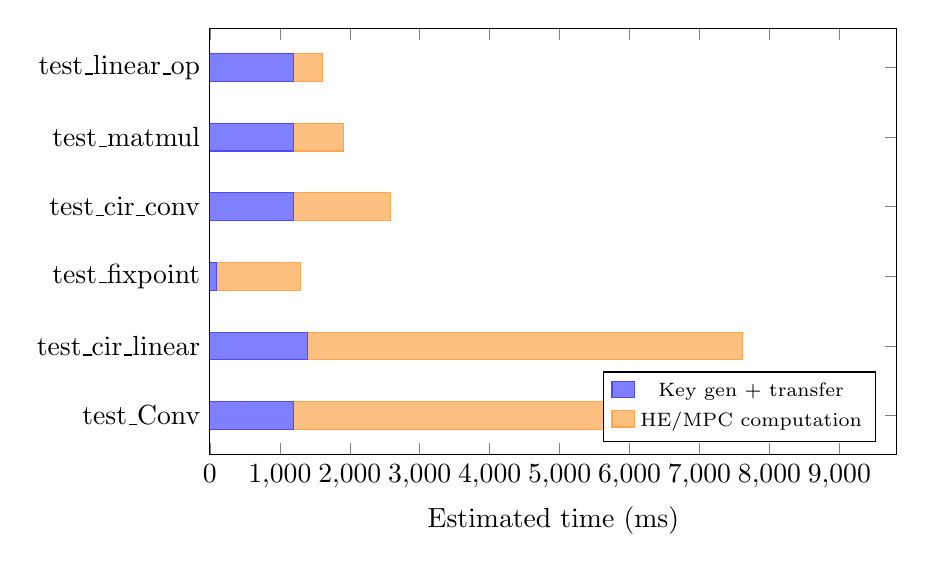
\begin{tikzpicture}
\begin{axis}[
    xbar stacked,
    width=0.85\textwidth,
    height=7cm,
    xlabel={Estimated time (ms)},
    symbolic y coords={
      {test\_linear\_op},
      {test\_matmul},
      {test\_cir\_conv},
      {test\_fixpoint},
      {test\_cir\_linear},
      {test\_Conv}
    },
    ytick=data,
    y dir=reverse,
    xmin=0,
    bar width=10pt,
    legend style={at={(0.97,0.03)}, anchor=south east, font=\scriptsize},
    enlarge y limits={abs=0.5cm},
]
\addplot[fill=blue!50, draw=blue!70] coordinates {
    (1200,{test\_linear\_op})
    (1200,{test\_matmul})
    (1200,{test\_cir\_conv})
    (100,{test\_fixpoint})
    (1400,{test\_cir\_linear})
    (1200,{test\_Conv})
};
\addlegendentry{Key gen + transfer}
\addplot[fill=orange!50, draw=orange!70] coordinates {
    (410,{test\_linear\_op})
    (711,{test\_matmul})
    (1385,{test\_cir\_conv})
    (1201,{test\_fixpoint})
    (6212,{test\_cir\_linear})
    (7729,{test\_Conv})
};
\addlegendentry{HE/MPC computation}
\end{axis}
\end{tikzpicture}
\caption{Estimated timing decomposition. Key generation + transfer is a fixed overhead ($\sim$1.2\,s for HE tests, $\sim$100\,ms for OT-only \texttt{test\_fixpoint}). The computation phase scales with the number of HE rotations or OT rounds. Estimates based on \texttt{test\_linear\_operator} establishing the key-gen baseline.}
\label{fig:timing-decomposition}
\end{figure}

\subsection{Coefficient of Variation Analysis}

\begin{figure}[ht]
\centering
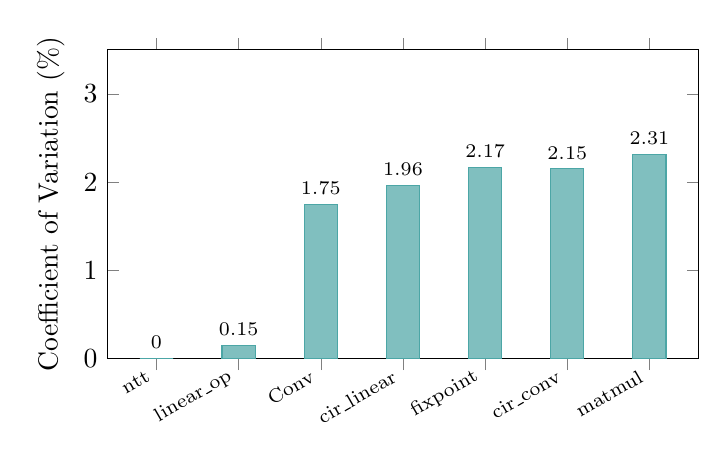
\begin{tikzpicture}
\begin{axis}[
    ybar,
    width=0.75\textwidth,
    height=5.5cm,
    ylabel={Coefficient of Variation (\%)},
    symbolic x coords={
      {ntt},
      {linear\_op},
      {Conv},
      {cir\_linear},
      {fixpoint},
      {cir\_conv},
      {matmul}
    },
    xtick=data,
    x tick label style={rotate=30, anchor=east, font=\scriptsize},
    ymin=0,
    ymax=3.5,
    bar width=12pt,
    nodes near coords,
    every node near coord/.append style={font=\scriptsize},
    enlarge x limits=0.1,
]
\addplot[fill=teal!50, draw=teal!70] coordinates {
    ({ntt}, 0.0)
    ({linear\_op}, 0.15)
    ({Conv}, 1.75)
    ({cir\_linear}, 1.96)
    ({fixpoint}, 2.17)
    ({cir\_conv}, 2.15)
    ({matmul}, 2.31)
};
\end{axis}
\end{tikzpicture}
\caption{Coefficient of variation (CV = $\sigma / \mu \times 100$) for each test. All tests show CV $< 2.5$\%, confirming that single-machine localhost benchmarks produce stable, reproducible measurements. The near-zero CV of \texttt{test\_linear\_operator} (0.15\%) reflects the deterministic nature of SEAL key generation and HE multiply.}
\label{fig:cv-analysis}
\end{figure}

\subsection{Comparison with Published Results}\label{sec:comparison}

The BLB paper reports end-to-end inference timings for full Transformer models (BERT-base, BERT-large, GPT2-base) under realistic network conditions.
We reproduce these results here (from Table~9 of the paper) and contextualize the gap between our local primitive-level benchmarks and the paper's system-level numbers.

\subsubsection{Paper's Experimental Setup}

The published BLB results were obtained on substantially different hardware and network conditions than our testbed:

\begin{table}[ht]
\centering
\caption{Hardware and network comparison: our testbed vs.\ the BLB paper}
\label{tab:hw-comparison}
\begin{tabular}{lll}
\toprule
 & \textbf{Our Testbed} & \textbf{BLB Paper} \\
\midrule
CPU & Xeon Silver 4208 @ 2.1\,GHz & Xeon Platinum 8558P @ 2.7\,GHz \\
Threads & 32 & 64 \\
GPU & None & NVIDIA A100 \\
Network & Localhost ($\sim$42\,$\mu$s RTT) & LAN / WAN (see below) \\
\bottomrule
\end{tabular}
\end{table}

The paper evaluates four network settings:
\begin{itemize}[nosep]
  \item \textbf{LAN}: 1\,Gbps bandwidth, 0.3\,ms RTT
  \item \textbf{WAN1}: 400\,Mbps bandwidth, 4\,ms RTT
  \item \textbf{WAN2}: 100\,Mbps bandwidth, 4\,ms RTT
  \item \textbf{WAN3}: 100\,Mbps bandwidth, 80\,ms RTT
\end{itemize}

\subsubsection{End-to-End Inference Results (Table~9)}

Table~\ref{tab:paper-e2e} reproduces the paper's end-to-end two-party inference timings for full Transformer models.
BLB is compared against BOLT~\cite{pang2024bolt}, Bumblebee~\cite{lu2023bumblebee}, and Iron~\cite{iron2022}.

\begin{table}[ht]
\centering
\caption{Published end-to-end 2PC inference times (from BLB Table~9). All times in minutes; communication in GB. ``/'' indicates data not reported.}
\label{tab:paper-e2e}
\resizebox{\textwidth}{!}{%
\begin{tabular}{llrrrr}
\toprule
\textbf{Model (tokens)} & \textbf{Protocol} & \textbf{LAN} & \textbf{WAN2} & \textbf{WAN3} & \textbf{Comm (GB)} \\
\midrule
\multirow{2}{*}{GPT2-base (64)}
  & BLB CPU  & 4.0  & 6.8   & 10.2  & 1.5  \\
  & BLB GPU  & 2.0  & 3.9   & 8.1   & 1.5  \\
\midrule
\multirow{5}{*}{BERT-base (128)}
  & BLB CPU    & 6.1   & 10.5  & 17.2   & 3.0   \\
  & BLB GPU    & 2.5   & 6.6   & 13.2   & 3.0   \\
  & BOLT       & 22.1  & 85.0  & 130.0  & 63.6  \\
  & Bumblebee  & 5.0   & 12.3  & 22.1   & 5.8   \\
  & Iron       & 66.7  & /     & /      & /     \\
\midrule
\multirow{4}{*}{BERT-large (128)}
  & BLB CPU    & 15.1  & 29.0  & 37.7   & 7.8   \\
  & BLB GPU    & 6.6   & 16.2  & 24.9   & 7.8   \\
  & BOLT       & 57.6  & 222.0 & 274.4  & 158.9 \\
  & Bumblebee  & 10.6  & 32.4  & 51.3   & 15.2  \\
\bottomrule
\end{tabular}%
}
\end{table}

Key observations from the published results:
\begin{itemize}[nosep]
  \item BLB GPU achieves a \textbf{2--2.5$\times$ speedup} over BLB CPU on LAN, with the gap narrowing under WAN conditions as network latency dominates.
  \item BLB CPU is competitive with Bumblebee on BERT-base (6.1\,min vs.\ 5.0\,min on LAN) while using \textbf{48\% less communication} (3.0\,GB vs.\ 5.8\,GB).
  \item Under high-latency WAN3 conditions, BLB's communication advantage becomes decisive: BLB CPU runs BERT-base in 17.2\,min vs.\ BOLT's 130.0\,min ($7.6\times$ faster).
  \item BERT-large end-to-end takes 15.1\,min (BLB CPU) to 6.6\,min (BLB GPU) on LAN, vs.\ 57.6\,min for BOLT --- a $3.8$--$8.7\times$ improvement.
\end{itemize}

\subsubsection{Communication Breakdown (Figure~11)}

The BLB paper's Figure~11 provides a detailed communication breakdown for BERT-base inference, highlighting the sources of BLB's communication savings:

\begin{table}[ht]
\centering
\caption{Communication reduction in BERT-base inference (from BLB Figure~11)}
\label{tab:comm-breakdown}
\begin{tabular}{lrrr}
\toprule
\textbf{Comparison} & \textbf{Baseline} & \textbf{BLB} & \textbf{Reduction} \\
\midrule
IKNP OT: BOLT $\to$ BLB          & 63.6\,GB & 15.0\,GB & $4.2\times$ \\
VOLE OT: Bumblebee $\to$ BLB     & 5.8\,GB  & 3.0\,GB  & $1.9\times$ \\
Truncation overhead               & non-zero & 0\,GB    & 100\% eliminated \\
HE/MPC conversion overhead        & baseline & --       & 55\% reduction \\
\bottomrule
\end{tabular}
\end{table}

BLB's communication savings come from three architectural innovations:
\begin{enumerate}[nosep]
  \item \textbf{Truncation-free fixed-point arithmetic}: BLB performs all CKKS computations in the HE domain and converts to secret shares only for nonlinear layers, completely eliminating the truncation protocol overhead that dominates BOLT's communication.
  \item \textbf{PrivCirNet block-circulant structure}: Reduces the number of HE ciphertext rotations, which in turn reduces the volume of key-switching material that must be communicated.
  \item \textbf{Optimized HE-to-MPC conversion}: The share-conversion protocol transfers only the necessary secret-share components, reducing conversion overhead by 55\% compared to prior approaches.
\end{enumerate}

\subsubsection{Bridging Our Benchmarks to Published Numbers}

Our local measurements (Section~\ref{tab:benchmarks}) exercise individual cryptographic primitives, not full Transformer inference.
The gap between our measurements and the paper's results is explained by several factors:

\begin{enumerate}[nosep]
  \item \textbf{Scope}: Our tests measure single operations (one HE matmul, one OT comparison batch). A BERT-base forward pass comprises 12 Transformer blocks, each containing attention (4 matmuls + softmax), layer normalization, and a 2-layer FFN --- hundreds of HE and OT operations in sequence.
  \item \textbf{Hardware}: The Xeon Platinum 8558P (2.7\,GHz, 64 threads) used in the paper is substantially faster than our Xeon Silver 4208 (2.1\,GHz, 32 threads), providing roughly $2\times$ the computational throughput for parallelizable HE operations.
  \item \textbf{GPU acceleration}: The paper's GPU results use an NVIDIA A100 for HE polynomial arithmetic via PhantomFHE, achieving 2--2.5$\times$ additional speedup. We have no GPU and cannot run the GPU code paths (\texttt{test\_HE}, \texttt{testHEGPU}, \texttt{testFFN}).
  \item \textbf{Network}: Our localhost measurements (42\,$\mu$s RTT) do not capture the communication overhead that is a major factor under WAN conditions. The paper's WAN3 setting (100\,Mbps, 80\,ms RTT) adds minutes of network transfer time for multi-GB communication volumes.
  \item \textbf{Extrapolation}: A rough lower-bound estimate for BERT-base on our hardware: 12 blocks $\times$ ($\sim$4 matmuls at 1.9\,s + OT nonlinear at $\sim$1.3\,s) $\approx$ 107\,s $\approx$ 1.8\,min of pure computation. The paper reports 6.1\,min on LAN with faster hardware, suggesting significant additional overhead from key management, share conversion, and protocol coordination not captured by our isolated tests.
\end{enumerate}

\subsection{Limitations}

\begin{itemize}[nosep]
  \item \textbf{Primitive-level only}: Our benchmarks measure individual cryptographic primitives on a single machine, not end-to-end Transformer inference. The published BLB results use different hardware (Xeon Platinum 8558P + A100 GPU) and measure full BERT/GPT2 inference across realistic network conditions.
  \item \textbf{GPU tests}: \texttt{test\_HE}, \texttt{testHEGPU}, and \texttt{testFFN} require an NVIDIA GPU and could not be validated. A GPU-enabled Docker image (\texttt{v1.0-gpu}) is prepared but untested.
  \item \textbf{Communication bytes}: Only \texttt{test\_fixpoint} reliably reports communication volume. The other tests do not print the \texttt{total data sent} line, so communication overhead for HE operations is not captured. A future instrumentation pass should add structured logging to the NetIO layer.
  \item \textbf{Localhost only}: All measurements are on loopback (RTT $\approx 42\,\mu$s). WAN latency and bandwidth effects are not captured. The \texttt{throttle.sh} utility can simulate WAN conditions, but true two-machine benchmarks with the aldebaran--maia link (RTT $\approx 203\,\mu$s) would be more informative.
  \item \textbf{No phase-level instrumentation}: The timing decomposition (Figure~\ref{fig:timing-decomposition}) is estimated from the \texttt{test\_linear\_operator} baseline, not measured directly. Adding \texttt{std::chrono} instrumentation inside the test binaries would enable precise phase breakdown.
  \item \textbf{Single parameter set}: Each test runs with its default parameters. A parameter sweep (varying polynomial degree $N$, number of channels, block size) would better characterize scaling behavior.
\end{itemize}
